% Source-bound manuscript candidate; scientific publication review is separate from build success.
\documentclass[aps,prd,onecolumn,11pt,nofootinbib,notitlepage]{revtex4-2}
\usepackage[T1]{fontenc}
\usepackage{amsmath,amssymb,bm,booktabs,graphicx}
\usepackage[colorlinks=true,linkcolor=blue,citecolor=blue,urlcolor=blue]{hyperref}
\setlength{\tabcolsep}{7pt}
\newcommand{\R}{\mathbb R}
\newcommand{\tr}{\operatorname{tr}}
\newcommand{\col}{\operatorname{col}}
\newcommand{\rank}{\operatorname{rank}}
\newcommand{\CommonMin}{3.117720}
\newcommand{\CommonMax}{3.118388}
\newcommand{\RawMin}{59.572829}
\newcommand{\RawMax}{59.592192}
\newcommand{\NominalAngle}{0.03854}
\newcommand{\ExtensionAngle}{3.6284\times10^{-5}}
\newcommand{\ExtensionWeight}{7955.99}

\begin{document}
\title{Finite-bandpass CMB identifiability with bounded foreground moments}
\author{}
\noaffiliation
\begin{abstract}
Frequency separation of the cosmic microwave background depends on the foreground class admitted by the analysis. We examine seven released Planck passband responses acting on the complete signed $E_2,E_3,B_2,B_3$ harmonic carrier. The declared first-order synchrotron--dust class leaves all 24 target coordinates spectrally identifiable in the finite model. Adding four free second-order moment maps gives a $7\times9$ nuisance response of resolved rank seven and removes the entire target quotient. A fixed joint quadratic coefficient bound nevertheless gives a sharp compensation frontier. We state the minimum compensator, the complete compatible target set and its coefficient fibres, retaining the two nuisance null directions. The stored minimum budget for a unit target displacement is $\CommonMin$--$\CommonMax$ in a common column-normalized metric, and $\RawMin$--$\RawMax$ in a separately declared raw-coordinate metric. A single compensator has radius $\rho/\ell_M$; two foregrounds, each bounded by $\rho$, can hide a separation as large as $2\rho/\ell_M$. These conclusions concern fixed finite response matrices and free signed moments. They supply no observed CMB amplitude, physical foreground bound or noise-calibrated region.
\end{abstract}
\maketitle

\section{The foreground class determines the question}

A calibrated frequency map responds to the CMB and to foreground emission after spectral averaging. Averaging spectra with different parameters introduces additional spectral shapes, as made explicit by the moment expansion of Chluba, Hill and Abitbol~\cite{Chluba2017}. Constrained linear combinations preserve a target response while cancelling declared nuisance responses~\cite{Remazeilles2011}; constrained moment methods apply this construction to foreground moments~\cite{Remazeilles2021}. The possibility of such cancellation is a question about the chosen response space before it is a question about statistical precision.

We study that space for seven released Planck passbands and two nested, stipulated foreground classes. The first contains five synchrotron and dust columns. The second adds four second-order columns and allows their harmonic coefficients to vary independently. This enlarged linear class is a relaxation of a physical moment model. A positive intensity, a nonlinear component spectrum or a truncation remainder can impose relations absent from the relaxation. We do not infer those relations from a matrix rank.

The finite calculation has two distinct conclusions. With unrestricted second-order coefficients, the nuisance response spans every frequency row. With a specified bound on those coefficients, a target displacement has a nonzero minimum cost. We retain both statements, including the metric that defines the bound. No map fit is needed to formulate this question.

\section{Responses, harmonics and units}

The seven frequency rows are ordered as $030,044,070,100,143,217,353\mathrm{PSB}$. They use LFI RIMO R3.31 and HFI RIMO R3.00 response tables. The response normalization is the dipole-calibrated finite spectral model; the antenna-temperature and intensity-response distinction is retained~\cite{PlanckLFI2013}. For an intensity spectrum $S$ and CMB derivative $b_\nu=\partial B_\nu/\partial T|_{T_{\rm CMB}}$, the finite definition is
\begin{equation}
 R_i[S]=\frac{\operatorname{trapz}(\tau_i S,\nu_i)}{\operatorname{trapz}(\tau_i b_\nu,\nu_i)},\qquad
 a_i=R_i[b_\nu]=1.
 \label{eq:response}
\end{equation}
The trapezoids join the retained released nodes. This is a finite-node definition, without a continuous-passband error certificate. Two LFI frequency conventions, A and B, are crossed with three HFI transmission thresholds $10^{-7},10^{-8},10^{-6}$. A retains the released LFI frequencies; B applies the retained half-bin shift before all frequency-dependent factors. Their difference is a version-sensitivity diagnostic. The six models do not define a calibrated uncertainty distribution.

The synchrotron index is $\beta_s=-3$ in Rayleigh--Jeans temperature, the dust index is $\beta_d=1.5$, and the reference frequencies are $30$ and $353\,\mathrm{GHz}$. We use $T_d=20\,\mathrm K$, $T_{\rm CMB}=2.7255\,\mathrm K$ and $t=(T-T_d)/T_d$. The ordered response columns are
\begin{equation}
 F_1=(s,s_\beta,d,d_\beta,d_t),\qquad
 F_2=(s,s_\beta,d,d_\beta,d_t,s_{\beta\beta},d_{\beta\beta},d_{\beta t},d_{tt}).
 \label{eq:columns}
\end{equation}
Here the subscripts denote spectral derivatives at the stipulated pivots, rather than harmonic indices. Taylor factorials are absorbed into the free coefficients. The temperature second derivative is $T_d^2\partial_T^2$ at the pivot, not $(T\partial_T)^2$.

The target is the real signed carrier $s\in\R^{24}$ consisting of $E_2(5),E_3(7),B_2(5),B_3(7)$. Within each multipole the order is $m=0$, followed by $(\sqrt2\operatorname{Re},-\sqrt2\operatorname{Im})$ for each positive $m$. This is the retained real representation of the polarized harmonic coefficients. The $E$ and $B$ multipoles are derived from spin-two polarization using the retained convention; no new spin conversion or sign choice is applied here. A scalar temperature coefficient is a different observable and is not appended to this carrier. Neither a scalar power nor an unsigned amplitude replaces its signed coordinates.

All rows and components refer to one common source harmonic frame and one fixed convention. A change of frame must transform the full carrier consistently. We use no new observer-frame, matter-frame or cosmological transfer relation. Component-separated SMICA is a derived map, not an eighth independent frequency observation; actual component-specific spatial responses require separate evidence~\cite{Planck2018IV}.

For $F=F_2$, write
\begin{equation}
 Y=a s^{\mathsf T}+FU,\quad
 Y\in\R^{7\times24},\quad U\in\R^{9\times24},\quad a=\bm1_7.
 \label{eq:model}
\end{equation}
Frequency-major row flattening gives target operator $a\otimes I_{24}$ and nuisance operator $F\otimes I_{24}$. All moment coordinates are free and signed. $Y,s,U$ use the same harmonic-amplitude unit, for example $\mu\mathrm K_{\rm CMB}$; $F$ is dimensionless. There is no observed $Y$ in this experiment.

\section{Unrestricted spectral identifiability}

Let $P_F$ project onto the orthogonal complement of $\col(F)$ in the declared Euclidean channel coordinates. Then
\begin{equation}
 P_{F\otimes I_{24}}(a\otimes I_{24})=(P_Fa)\otimes I_{24}.
 \label{eq:quotient}
\end{equation}
Its target rank is 24 if $a\notin\col(F)$ and zero if $a\in\col(F)$. Thus the full carrier is retained or lost together in this separable finite response model. This statement does not identify the physical origin of a retained carrier.

In all six stored branches, $F_1$ has resolved nuisance rank five and augmented rank six, leaving target rank 24. The nine-column $F_2$ has resolved rank seven and augmented rank seven, leaving target rank zero. The numerical rank criteria apply to unit-column matrices: singular values at least $10^{-10}$ are resolved nonzero; values at most $10^{-12}$ are unresolved or zero under that criterion; intermediate values require an unresolved classification. A resolved finite rank is not an exact theorem about every physical passband. The nominal first-order principal-angle sine is about $\NominalAngle$, which already warns that algebraic retention alone does not establish useful separation with real noise.

\begin{table}[t]
\caption{Stored finite ranks for all six conventions. $r_j$ is the nuisance rank, $r_{j+a}$ the augmented rank including the CMB response, and $q_j$ the retained signed24 target rank. The ranks concern the stipulated finite matrices.}
\centering\begin{tabular}{lrrrrrr}
\toprule
Branch & $r_1$ & $r_{1+a}$ & $q_1$ & $r_2$ & $r_{2+a}$ & $q_2$ \\
\midrule
A\_BT\_1e-07 & 5 & 6 & 24 & 7 & 7 & 0 \\
A\_BT\_1e-08 & 5 & 6 & 24 & 7 & 7 & 0 \\
A\_BT\_1e-06 & 5 & 6 & 24 & 7 & 7 & 0 \\
B\_BT\_1e-07 & 5 & 6 & 24 & 7 & 7 & 0 \\
B\_BT\_1e-08 & 5 & 6 & 24 & 7 & 7 & 0 \\
B\_BT\_1e-06 & 5 & 6 & 24 & 7 & 7 & 0 \\
\bottomrule
\end{tabular}

\end{table}
\begin{figure}[t]
\centering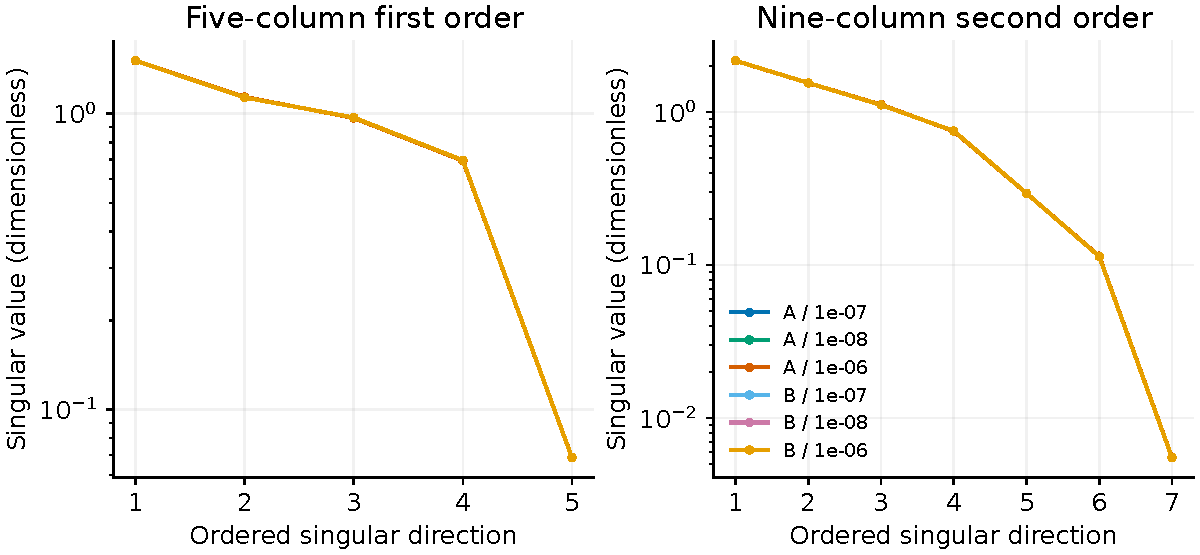
\includegraphics[width=.97\textwidth]{figures/response_spectra.pdf}
\caption{Retained nuisance singular spectra for the five-column first-order and nine-column second-order classes in all six conventions. Each nuisance column is normalized within its own branch, as in the retained response-rank calculation; this is distinct from the common coefficient metric used below. The number of resolved nuisance directions changes from five to seven. Channel-space dimension is seven. These spectra describe finite spectral geometry, without a noise covariance.}
\label{fig:spectra}
\end{figure}

\section{A fixed coefficient metric and the minimum compensator}

We impose the joint bound
\begin{equation}
 \|U\|_M^2=\tr(U^{\mathsf T}MU)\le\rho^2,\qquad M>0.
 \label{eq:budget}
\end{equation}
It covers all nine moment maps and all 24 signed coordinates together. The primary metric is fixed across all six branches: $M=\operatorname{diag}(d^2)$, where $d$ is the nominal A, $10^{-7}$ response column-scale vector,
\begin{align}
 d={}&(1.261652382369369,0.1777139521270542,1.1309894216176297,\nonumber\\
 &0.09451923139372441,0.04109240642871376,0.1151042544103929,\nonumber\\
 &0.07145402059880916,0.022520789584731377,0.09386151314750793).
\end{align}
This choice compares reference column-normalized moment amplitudes. It is a computational class definition, not a measured foreground prior or covariance. We separately consider $M=I_9$, which defines a different class. The budget $\rho$ has the target-amplitude unit.

For full-row-rank $F$ define
\begin{equation}
 K=FM^{-1}F^{\mathsf T},\qquad
 c_M=M^{-1}F^{\mathsf T}K^{-1}a,\qquad
 \ell_M^2=a^{\mathsf T}K^{-1}a.
 \label{eq:minimum}
\end{equation}
Since $K$ is positive definite, these quantities exist. Minimizing $c^{\mathsf T}Mc$ subject to $Fc=a$ gives $Mc=F^{\mathsf T}\lambda$ and $K\lambda=a$. Every solution is $c_M+n$, with $Fn=0$, and
\begin{equation}
 (c_M+n)^{\mathsf T}M(c_M+n)=\ell_M^2+n^{\mathsf T}Mn.
 \label{eq:orthogonality}
\end{equation}
This proves uniqueness and minimality. For a target displacement $v$, the minimum signed compensator is $-c_Mv^{\mathsf T}$ and its norm is $\ell_M\|v\|_2$.

The singular decomposition $FM^{-1/2}=U_f\operatorname{diag}(\sigma_i)V_f^{\mathsf T}$ gives
\begin{equation}
 \ell_M^2=\sum_{i=1}^7\frac{(u_i^{\mathsf T}a)^2}{\sigma_i^2}.
 \label{eq:singular}
\end{equation}
The cost depends on CMB alignment as well as the singular values. The vectors $v_i$ are whitened coefficient directions; their original-coordinate versions are $M^{-1/2}v_i$. Confusing these coordinate systems changes the stated nuisance directions.

\begin{table}[t]
\caption{Nominal A, $10^{-7}$ minimum compensator in original signed moment coordinates, with common metric scales $d_j$. Both columns solve $Fc=a$; their different minima follow from the different declared metrics. Coefficients and scales are dimensionless. Table values are rounded for display; full stored values accompany the source.}
\centering\begin{tabular}{lrrr}
\toprule
Moment & $d_j$ & $(c_M)_j$ & $(c_I)_j$ \\
\midrule
s & 1.26165 & 0.462241 & 0.457224 \\
s\_beta & 0.177714 & 1.00057 & 0.987669 \\
d & 1.13099 & 0.946754 & 0.93977 \\
d\_beta & 0.0945192 & -2.11365 & 8.83797 \\
d\_t & 0.0410924 & -6.80923 & -14.1702 \\
s\_betabeta & 0.115104 & 1.4828 & 1.43943 \\
d\_betabeta & 0.071454 & 36.5719 & 38.3879 \\
d\_beta\_t & 0.0225208 & -49.2015 & -42.0275 \\
d\_tt & 0.0938615 & -0.479782 & 5.3136 \\
\bottomrule
\end{tabular}

\label{tab:coefficients}
\end{table}
\begin{figure}[t]
\centering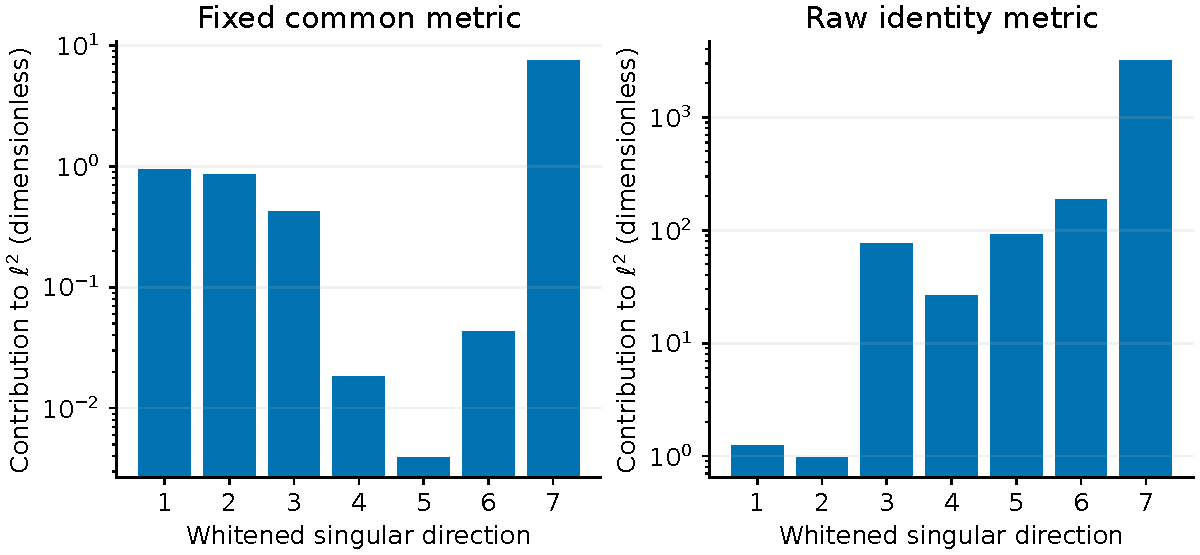
\includegraphics[width=.97\textwidth]{figures/budget_contributions.pdf}
\caption{Nominal A, $10^{-7}$ contributions $(u_i^{\mathsf T}a)^2/\sigma_i^2$ to the minimum squared budget in Eq.~\eqref{eq:singular}, for each metric's own whitened singular directions. The smallest singular direction dominates the cost in this example. The logarithmic ordinate preserves the smaller contributions. This is spectral alignment in a computational coefficient class, not measured foreground power.}
\label{fig:contributions}
\end{figure}

\section{The complete target set and its fibres}

For a specified $Y$ and proposed $s$, the minimum-budget foreground is
\begin{equation}
 U_s=M^{-1}F^{\mathsf T}K^{-1}(Y-as^{\mathsf T}),\quad
 J(s)=\tr[(Y-as^{\mathsf T})^{\mathsf T}K^{-1}(Y-as^{\mathsf T})].
 \label{eq:conditional}
\end{equation}
Let
\begin{equation}
 s_0=\frac{Y^{\mathsf T}K^{-1}a}{\ell_M^2},\qquad
 J_0=\tr[(Y-as_0^{\mathsf T})^{\mathsf T}K^{-1}(Y-as_0^{\mathsf T})].
 \label{eq:center}
\end{equation}
Completing the square gives the full identified set
\begin{equation}
 \boxed{\mathcal S_\rho(Y)=\{s\in\R^{24}:J_0+\ell_M^2\|s-s_0\|_2^2\le\rho^2\}.}
 \label{eq:set}
\end{equation}
It is empty for $\rho^2<J_0$, a singleton at equality, and otherwise a closed ball of radius $\sqrt{\rho^2-J_0}/\ell_M$. These are exact conditional statements. In numerical work, $J_0$ should be evaluated from the residual in Eq.~\eqref{eq:center}; an unresolved comparison with $\rho^2$ cannot be reported as a certified boundary. No likelihood or coverage statement enters this construction.

The numerical representation uses serialized binary64 center and radius parameters interpreted as exact real numbers. For a resolved ball, let $c_*,J_*$ denote the exact finite-input center and minimum cost, and let $\widehat c,\widehat r$ be the returned parameters. With $\delta_c=\|\widehat c-c_*\|$, the all-direction sphere error is
\begin{equation}
 D=\left|J_*+\ell_M^2(\delta_c^2+\widehat r^2)-\rho^2\right|
       +2\ell_M^2\widehat r\delta_c.
\end{equation}
The retained numerical policy requires its uncertainty-enlarged bound divided by $\max(\rho^2,J_*)$ to be at most $10^{-9}$ for admitted positive-radius balls. Unresolved geometry or radius quantization retains a numerical hold. This policy concerns the real set parameterized by $\widehat c,\widehat r$. Arbitrary later rounded evaluation of $\widehat c+\widehat r u$ is a separate floating-point operation and has no universal boundary guarantee. The particular exported attainment witnesses retain their own norm and reconstruction checks. This is a finite-input numerical policy, not a general interval certificate.

The coefficient fibre must also be retained. Set $G=F\operatorname{diag}(d)^{-1}$ and choose a two-column orthonormal basis $N_z$ of $\ker G$. In original moment coordinates,
\begin{equation}
 N_c=\operatorname{diag}(d)^{-1}N_z,\qquad FN_c=0,\qquad N_c^{\mathsf T}MN_c=I_2.
 \label{eq:null}
\end{equation}
Every coefficient array realizing the same $Y,s$ is $U_s+N_cZ$, with $Z\in\R^{2\times24}$. The orthogonality in Eq.~\eqref{eq:orthogonality}, applied to each column, gives
\begin{equation}
 \|U_s+N_cZ\|_M^2=J(s)+\|Z\|_F^2.
 \label{eq:fibre}
\end{equation}
Thus each admissible target has its complete null-coordinate fibre $\|Z\|_F^2\le\rho^2-J(s)$. For the raw metric the same construction uses its own whitening. A numerical basis is not unique; the coefficient nullspace, its metric and its lifted action are the invariant content.

\section{Sharp frontiers and coordinate invariance}

For zero data, $s_0=0$ and $J_0=0$. One bounded foreground hides a target displacement precisely when $\|v\|\le\rho/\ell_M$. For two foregrounds each bounded by $\rho$, choose
\begin{equation}
 s_1=v/2,\quad s_2=-v/2,\quad
 U_1=-c_Mv^{\mathsf T}/2,\quad U_2=c_Mv^{\mathsf T}/2.
\end{equation}
Both give $Y=0$, and each has budget $\ell_M\|v\|/2$. Conversely, $F(U_2-U_1)=a(s_1-s_2)^{\mathsf T}$ and minimality imply
\begin{equation}
 \ell_M\|s_1-s_2\|\le\|U_2-U_1\|_M\le2\rho.
\end{equation}
The pairwise bound is attained. At a fixed nonempty generic $Y$, its diameter is $2\sqrt{\rho^2-J_0}/\ell_M$, which need not equal $2\rho/\ell_M$.

Nonzero column rescaling is a coordinate change only when the metric is transported with it: $F'=FS$, $U'=S^{-1}U$, $M'=S^{\mathsf T}MS$ for nonsingular diagonal $S$. Then $K$, $\ell_M$ and the target set are unchanged. A fixed orthogonal right transformation $O$ of the carrier sends $(Y,U,s)$ to $(YO,UO,O^{\mathsf T}s)$ and preserves the budget. The set transforms as $O^{\mathsf T}\mathcal S_\rho(Y)$. Arbitrary nonorthogonal transformations do not preserve the Euclidean carrier norm without also transporting its metric.

\begin{table}[t]
\caption{Source-bound six-branch minimum budgets and frontier slopes. The common metric is fixed across branches; the identity metric defines a different coefficient class. These are finite algebraic quantities, not measured CMB amplitudes.}
\centering
\begin{tabular}{lrrrr}
\toprule
Branch & $\ell_M$ & $1/\ell_M$ & $2/\ell_M$ & $\ell_I$ \\
\midrule
A\_BT\_1e-07 & 3.118381 & 0.320679 & 0.641358 & 59.592105 \\
A\_BT\_1e-08 & 3.118381 & 0.320679 & 0.641358 & 59.592092 \\
A\_BT\_1e-06 & 3.118388 & 0.320678 & 0.641357 & 59.592192 \\
B\_BT\_1e-07 & 3.117720 & 0.320747 & 0.641494 & 59.572842 \\
B\_BT\_1e-08 & 3.117720 & 0.320747 & 0.641494 & 59.572829 \\
B\_BT\_1e-06 & 3.117727 & 0.320747 & 0.641493 & 59.572929 \\
\bottomrule
\end{tabular}

\label{tab:budgets}
\end{table}

The retained values give $\ell_M=\CommonMin$--$\CommonMax$ for the common metric and $\ell_I=\RawMin$--$\RawMax$ for the raw metric. The change is a change in the bounded class. Within each metric, the branch envelope measures the sensitivity of these six finite conventions. Neither comparison establishes a physical foreground amplitude bound.

\begin{figure}[t]
\centering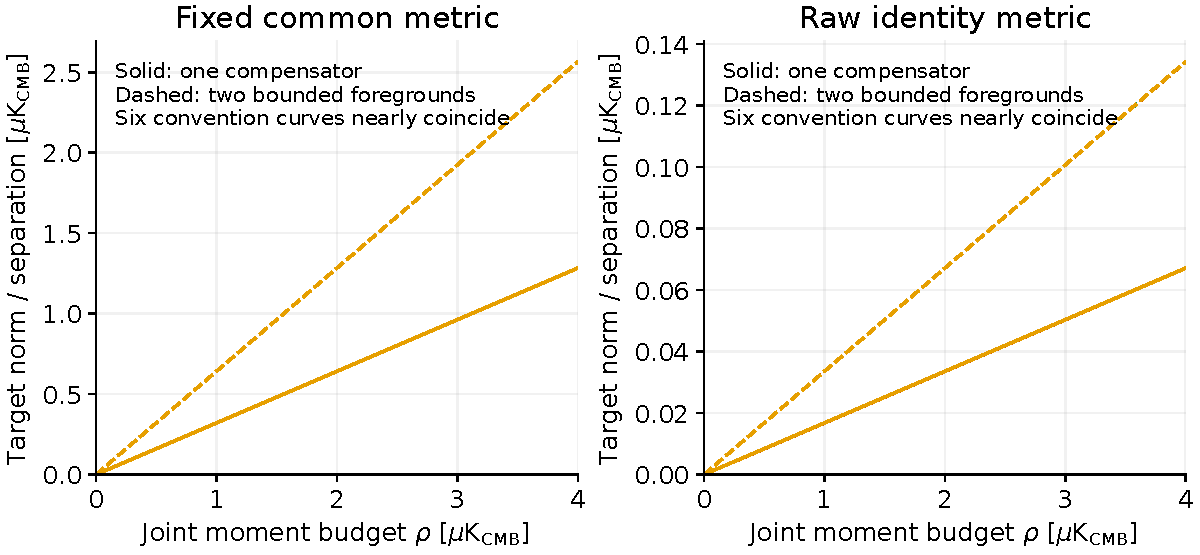
\includegraphics[width=.97\textwidth]{figures/frontier.pdf}
\caption{Sharp compensation frontiers in the declared joint coefficient class. Solid curves give the one-compensator target radius $\rho/\ell$; dashed curves give the largest possible separation for two foregrounds each bounded by $\rho$. Each panel contains all six response conventions, whose slopes nearly coincide. The two panels use different metrics and hence different bounded classes. The horizontal range is a chosen illustrative budget range, not an observed foreground amplitude. All curves use stored minimum costs and slopes.}
\label{fig:frontier}
\end{figure}

\section{An additional finite-response comparison}

A separately checked WMAP--Planck extension reuses the seven nominal Planck rows and adds stipulated WMAP response averages. It distinguishes 12 instrument-band-average rows from 17 differencing-assembly response rows; the latter are not 17 independent frequencies. Across its 12 paired conventions, the nine-column nuisance matrix has resolved rank nine and the augmented matrix rank ten in both row constructions, retaining all 24 target coordinates in the finite model. The stored independent check gives a minimum principal-angle sine of approximately $\ExtensionAngle$ and maximum Euclidean weight norm $\ExtensionWeight$. This is a severe conditioning warning. There is no supplied actual noise law or polarized spatial-response model from which to establish useful sky separation. The extension changes the finite response geometry; it does not replace the seven-row result or the coefficient class studied above.

\section{Physical interpretation and remaining inputs}

At zero budget, $U=0$ and compatible data must equal $as^{\mathsf T}$. Exact pure-target data therefore give a singleton at $\rho=0$, and a full ball at positive budget. As $\rho$ grows without bound, the unrestricted second-order loss of the target quotient is recovered. These limits give a direct reading of the frontier: it is the cost of compensation in a stipulated coefficient class.

The independent signed coordinates do not enforce physical realizability. Positivity of an underlying intensity does not require positive polarization harmonics or positive derivative moments. A physical restriction needs supplied moment magnitudes and couplings, a truncation-remainder bound, component-specific spatial responses, and a justified metric and radius. A noise-calibrated region additionally needs the actual joint noise and calibration law. A nuisance with the exact CMB blackbody response remains spectrally confounded.

No observed target tensor or physical anisotropy parameter is measured here. In particular, full-tensor nonlinear quantities remain undefined in sectors where the target is unobserved or the required denominators are absent. A frequency axis supplies no depth information. The finite response results do not infer a local or global tilt, identify a Bianchi family, or validate a native cosmological solver. Their use is to specify which additional response directions or physically justified foreground restrictions an observational analysis must supply.

\bibliographystyle{apsrev4-2}
\bibliography{references}
\end{document}
